\documentclass[aspectratio=169]{beamer}
\usepackage{xspace}
\usepackage{tikz}
\usepackage{url,color,minted}
\usepackage{pgf,pgflibraryshapes}
\usetikzlibrary{shadows,arrows}

\usepackage[siunitx]{circuitikz}

\tikzstyle{linedot} = [draw, thick, color=black!50, dotted]
\tikzstyle{linepart} = [draw, thick, color=black!50, dashed]
\tikzstyle{linegrey} = [draw, thick, color=black!50]
\tikzstyle{linesolid} = [draw, thick, color=black, -latex', align=center]

\tikzstyle{ellipsesolid} = [draw, ultra thick, color=blue, ellipse, -latex', align=center]



\graphicspath{{./fig/},{../circuit/}}

\mode<presentation> { % handout / presentation
	\usetheme{Darmstadt}
	\setbeamertemplate{navigation symbols}{}
	\defbeamertemplate*{footline}{infolines2 theme}{
	  \leavevmode%
	  \hbox{%
	  \begin{beamercolorbox}[wd=\paperwidth,ht=2.25ex,dp=1ex,right]{quaternary}%	 
	    \insertframenumber{} / \inserttotalframenumber\hspace*{1ex} 
	  \end{beamercolorbox}}%
	  \vskip0pt%
	}
  
  \setbeamercolor*{palette primary}{use=structure,fg=black,bg=structure.fg!40!white}
  \setbeamercolor*{palette secondary}{use=structure,fg=black,bg=structure.fg!60!white}
  \setbeamercolor*{palette tertiary}{use=structure,fg=black,bg=structure.fg!90!white}
  \setbeamercolor*{palette quaternary}{fg=white,bg=black}

  \setbeamercolor*{sidebar}{use=structure,bg=structure.fg}

  \setbeamercolor*{palette sidebar primary}{use=structure,fg=structure.fg!10}
  \setbeamercolor*{palette sidebar secondary}{fg=white}
  \setbeamercolor*{palette sidebar tertiary}{use=structure,fg=structure.fg!50}
  \setbeamercolor*{palette sidebar quaternary}{fg=white}

  \setbeamercolor*{titlelike}{parent=palette primary}

  \setbeamercolor*{separation line}{}
  \setbeamercolor*{fine separation line}{}
}

\pgfdeclareimage[height=1cm]{logoRIOT}{fig/RIOT_logo.png}
\pgfdeclareimage[height=1cm]{logoSTM32}{fig/STM32_logo.png}

\title[Lecture 1]{How to use a Photocell with RIOT}
\subtitle{using an STM32 Nucleo-64 F401RE development board}

\author[I.Chatzigiannakis]{Ioannis Chatzigiannakis}

\institute{\url{https://github.com/ichatz/riotos-apps}}

\date{}

\logo{\pgfuseimage{logoRIOT}\pgfuseimage{logoSTM32}}

\begin{document}

{
\setbeamercolor{upper separation line head}{fg=white, bg=white}
\setbeamercolor{lower separation line head}{fg=white, bg=white}
\setbeamercolor{title in head/foot}{fg=white, bg=white}
\setbeamercolor{institute in head/foot}{fg=white, bg=white}
\setbeamercolor{date in head/foot}{fg=white, bg=white}
\setbeamercolor{author in head/foot}{fg=white, bg=white}
\setbeamercolor{date in head/foot}{fg=white, bg=white}
\setbeamercolor{section in head/foot}{fg=white, bg=white}
\setbeamercolor{subsection in head/foot}{fg=white, bg=white}
\setbeamercolor{subsubsection in head/foot}{fg=white, bg=white}
\setbeamercolor{quaternary}{fg=white, bg=white}
\setbeamertemplate{headline}{}

\frame{\titlepage}

}

\section{How to use a Photocell with RIOT}

\subsection{}

%_____________________________________________________________
\begin{frame}{}

\begin{block}{}
Measure the intensity of ambient light with an \href{https://www.st.com/en/evaluation-tools/nucleo-f401re.html}{STM32 Nucleo-64 F401RE development board} and the \href{https://github.com/RIOT-OS/RIOT}{RIOT operating system}.
\end{block}

\bigskip

Required hardware components:

\begin{itemize}
	
\item STM32 Nucleo-64 F401RE

\item Breadboard

\item $1K\Omega$ resistor

\item Photocell (or Photoresistor, or Light-Dependent-Resistor LDR)

\item 3 Male to male jumper wires

\end{itemize}
\end{frame}


%_____________________________________________________________
\begin{frame}{}
\begin{columns}

\column{.65\textwidth}
\begin{itemize}

\item The photocell is a light-controlled variable resistor:

\begin{itemize}

\item \alert{When struck by light} -- resistance decreases.

\item \alert{In absence of light} -- resistance increases.

\end{itemize}

\item Measure the variable resistor $\rightarrow$ measure intensity of ambient light.

\item Measure a variable resistance:

\begin{itemize}

\item Connect one end to power (+5V),

\item Connect the other to a pull-down resistor ($1K\Omega$) to ground (GND).

\item Connect the point INPUT to the analog input of the STM32 board.

\end{itemize}

\item The pull-down resistor depends on:

\begin{itemize}

\item Input voltage (5V or 3.3V or \ldots).

\item Intensity of ambient light.

\end{itemize}



\end{itemize}

\column{.35\textwidth}
\begin{block}{}
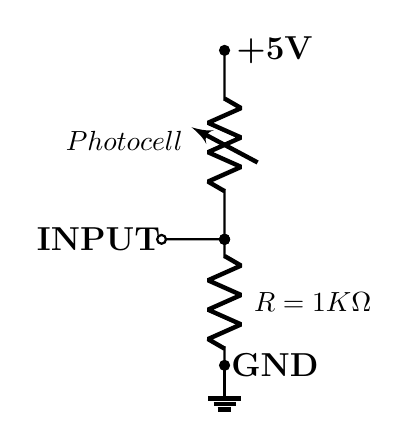
\begin{tikzpicture}[scale=.8]
\draw[color=black, thick]
    (0,0) to [short,o-] (1,0){} % Baseline for connection to ground
    % Input and ground
    (-1,0) node[]{\large{\textbf{INPUT}}}
    (1,0) node[circ]{}
    (1,0) to [R, *-*] (1,-2)
    (2.4,-1) node[]{$R=1K\Omega$}    
    (1,-2) node[ground]{}
    (1.8,-2) node[]{\large{\textbf{GND}}}
    (1,0) to [vR, l=$Photocell$, *-*] (1,3)
    (1.8,3) node[]{\large{\textbf{+5V}}};
\end{tikzpicture}
\end{block}
\vspace{1cm}

\end{columns}
\end{frame}


%_____________________________________________________________
\begin{frame}{}
\hspace*{1cm}
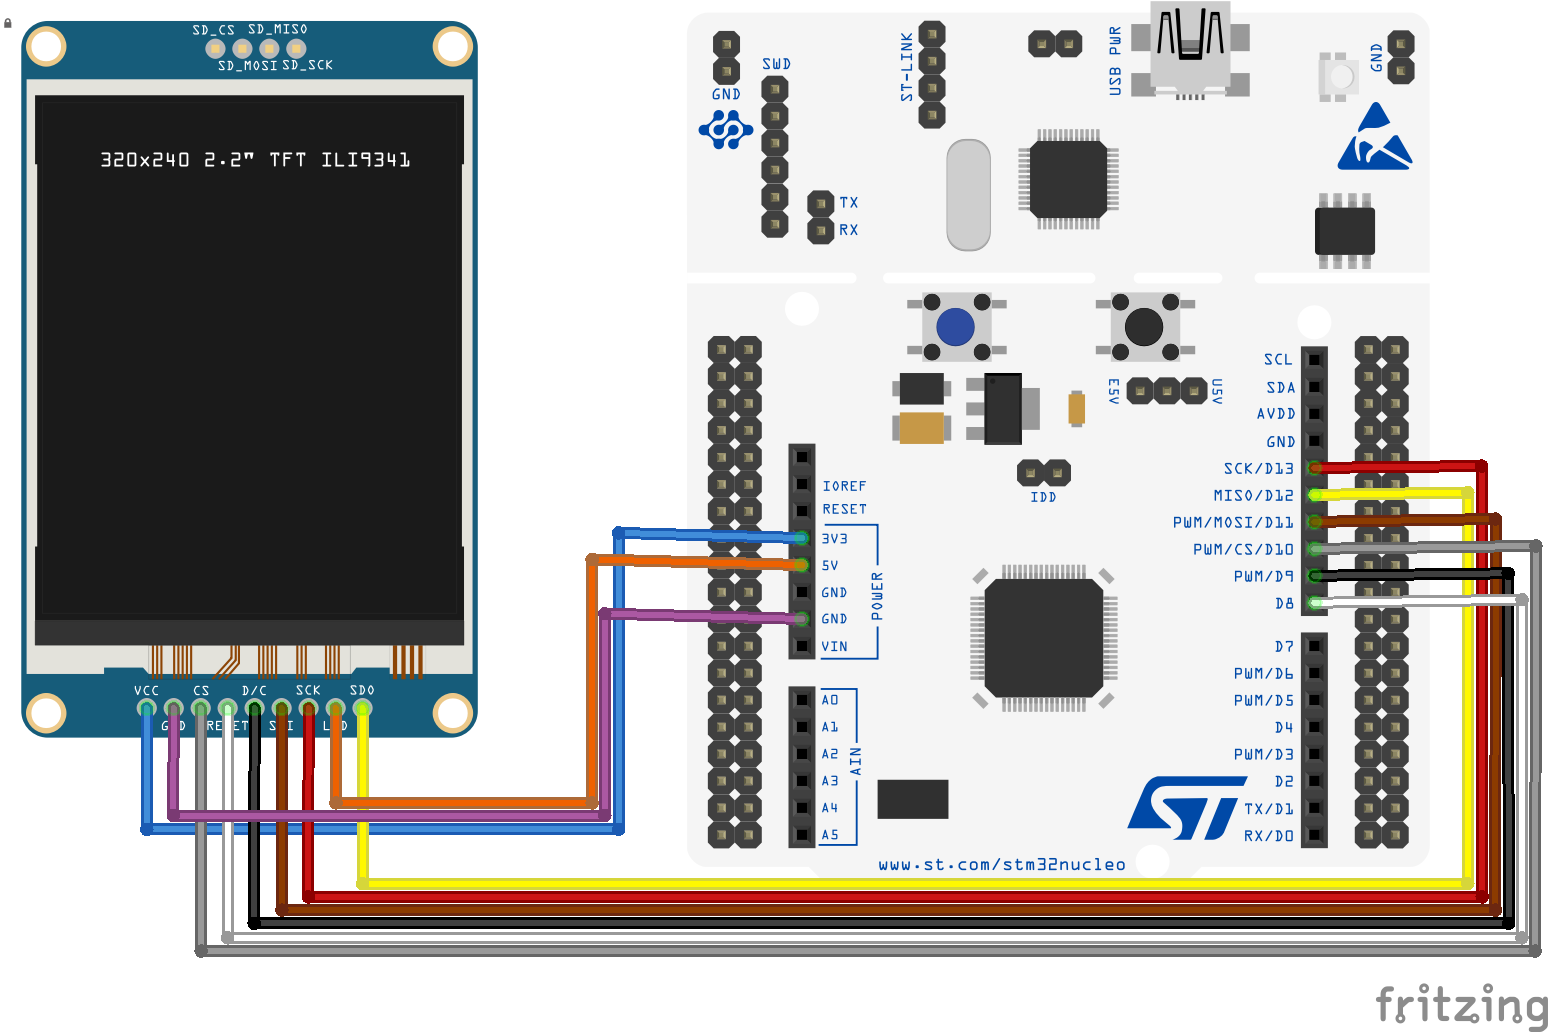
\includegraphics[width=.65\textwidth]{circuit_bb}
\end{frame}





%=============================================================
\subsection{STM32 Nucleo-64 F401RE development board}
\logo{\pgfuseimage{logoSTM32}}

%_____________________________________________________________
\begin{frame}{}
\begin{columns}

\column{.6\textwidth}

\begin{block}{}
The STM32 Nucleo-64 board provides an affordable and flexible way for users to try out new concepts and build prototypes by choosing from the various combinations of performance and power consumption features, provided by the STM32 microcontroller.
\end{block}

\bigskip

Highlights of the STM32F401RE MCU:

\begin{itemize}
	
\item 32-bit ARM Cortex-M4 processor

\item 512KB ROM Flash memory

\item 96KB SRAM data memory

\item Up to 84Mhz operating frequency

\item 42$\mu$A in sleep (stop mode) w/RTC

\end{itemize}

\column{.42\textwidth}
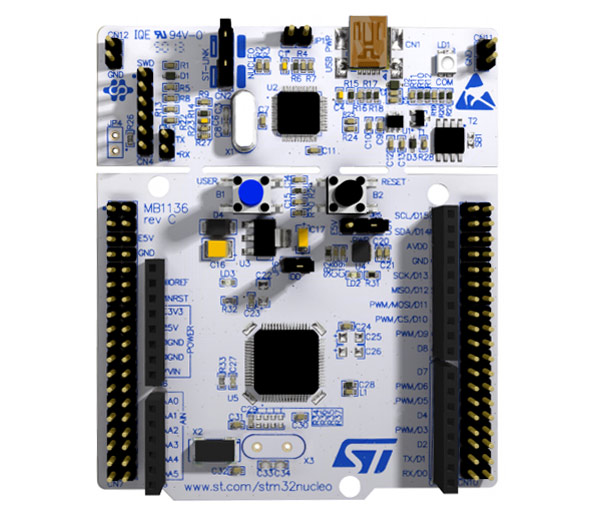
\includegraphics[width=\textwidth]{STM32-Nucleo-F401RE-board}

\end{columns}
\end{frame}

%_____________________________________________________________
\begin{frame}{}
\centering
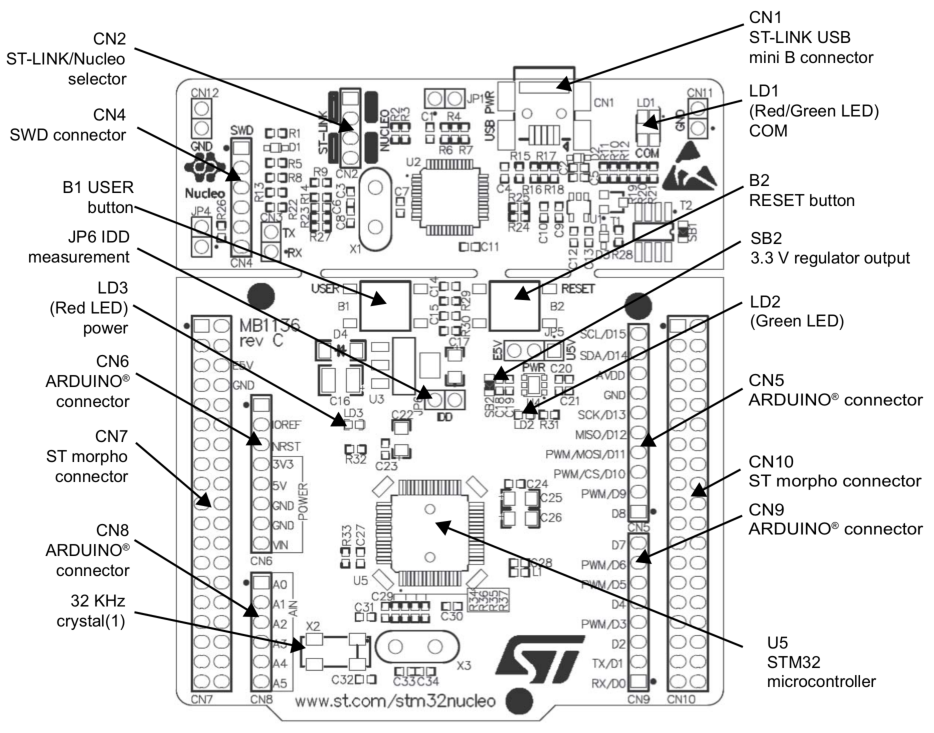
\includegraphics[height=\textheight]{stm32-nucleo64-boards-mb1136-stmicroelectronics}
\end{frame}


%_____________________________________________________________
\begin{frame}{STM32F401RE Architecture}
\centering
\begin{tikzpicture}
    
\node (img1) at (0,0) {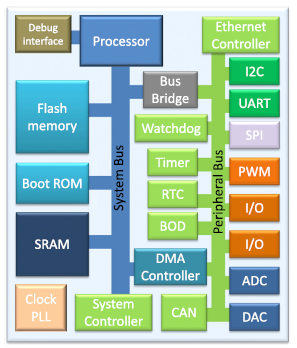
\includegraphics[width=.4\textwidth]{stm32f401re-schema}};

\node (img2) at (6.5,0) {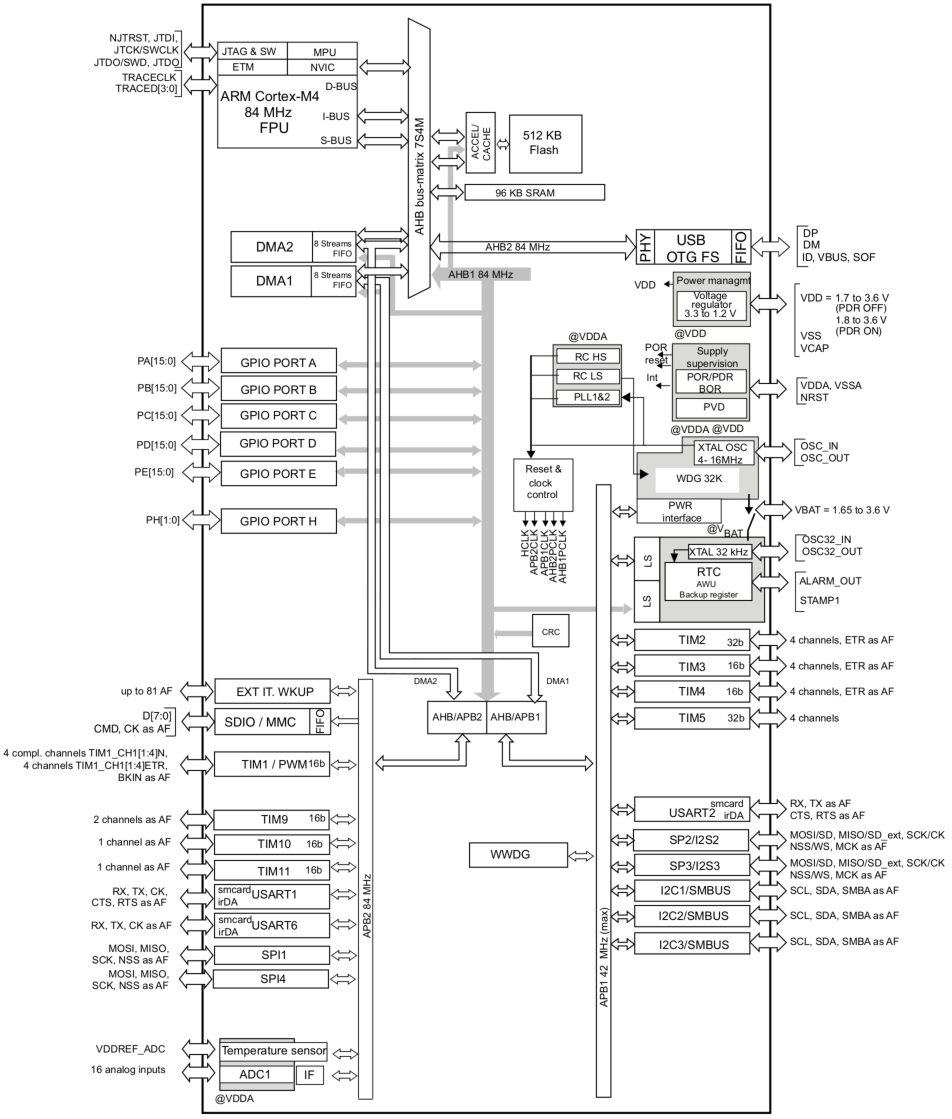
\includegraphics[height=.85\textheight]{stm32f401re-diagram}};

\node<1>[ellipsesolid, minimum width=40pt, minimum height=40pt] at (2, -1) {};
\node<1>[ellipsesolid, minimum width=30pt, minimum height=50pt] at (5.3, .7) {};

\node<2>[ellipsesolid, minimum width=40pt, minimum height=20pt] at (2, -2) {};
\node<2>[ellipsesolid, minimum width=30pt, minimum height=20pt] at (5.3, -3) {};

\node<3>[ellipsesolid, minimum width=40pt, minimum height=20pt] at (0.4, .2) {};
\node<3>[ellipsesolid, minimum width=30pt, minimum height=30pt] at (5.4, -1.5) {};

\node<4>[ellipsesolid, minimum width=70pt, minimum height=30pt] at (-0.6, 2.5) {};
\node<4>[ellipsesolid, minimum width=50pt, minimum height=30pt] at (5.4, 2.8) {};

\end{tikzpicture}
\end{frame}


%=============================================================
\subsection{The RIOT operating system}
\logo{\pgfuseimage{logoRIOT}}


%_____________________________________________________________
\begin{frame}{RIOT Architecture}
\begin{columns}

\column{.6\textwidth}
\begin{block}{}
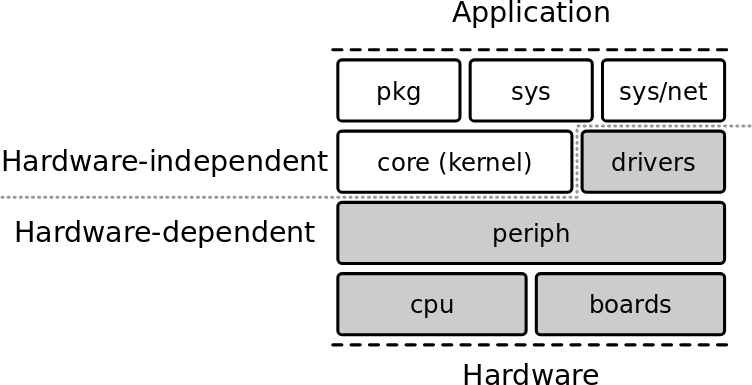
\includegraphics[width=\textwidth]{riot-architecture}
\end{block}

\column{.4\textwidth}

\textbf{Application logic\\
{\Large +} RIOT Kernel
{\Large +} RIOT Libraries}

\vspace{1.2cm}

\end{columns}

\vspace{.5cm}

\begin{itemize}

\item Generic API for peripherals (gpio, uart, spi, pwm, etc)

\begin{itemize}

\item same API for all architectures

\end{itemize}

\item CPU, Boards and Drivers: manufacturer specific

\end{itemize}

\vspace{2cm}
\end{frame}


%_____________________________________________________________
\begin{frame}[fragile]{Hardware Independent elements}
\begin{columns}

\column{.55\textwidth}
\begin{exampleblock}{Makefile}
\begin{minted}{c}
# name of application
APPLICATION = photocell

# Path to the RIOT base directory:
RIOTBASE ?= $(CURDIR)/../../RIOT

# RIOT features
FEATURES_REQUIRED += periph_adc

# Modules to include:
USEMODULE += analog_util
USEMODULE += xtimer
\end{minted}
\end{exampleblock}
%$

\column{.35\textwidth}

\vspace{3.5cm}

We specify the ADC as \alert{required} feature.

\bigskip

We also specify that we want to use two \alert{OS modules}.

\column{.1\textwidth}

\end{columns}
\vspace{2cm}
\end{frame}

%_____________________________________________________________
\begin{frame}[fragile]{Hardware Dependent elements}

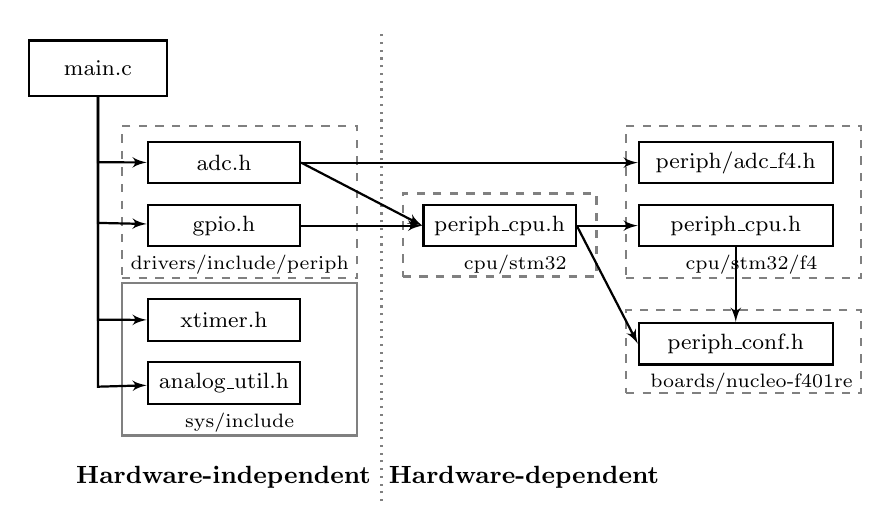
\begin{tikzpicture}

\node[linesolid, minimum width=50pt, minimum height=20pt] (main) at (-.6, 4) {\footnotesize main.c};



\node[linesolid, minimum width=55pt, minimum height=15pt] (adc) at (1, 2.8) {\footnotesize adc.h};
\node[linesolid, minimum width=55pt, minimum height=15pt] (gpio) at (1, 2) {\footnotesize gpio.h};
\node[linepart, minimum width=85pt, minimum height=55pt] at (1.2, 2.3) {};
\node at (1.2, 1.5) {\scriptsize drivers/include/periph};

\path [linesolid] (main.south) -- +(0, -.83) -- node [left] {} (adc);
\path [linesolid] (main.south) -- +(0, -1.6) -- node [left] {} (gpio);



\node[linesolid, minimum width=55pt, minimum height=15pt] (xtimer) at (1, 0.8) {\footnotesize xtimer.h};
\node[linesolid, minimum width=55pt, minimum height=15pt] (analogutil) at (1, 0) {\footnotesize analog\_util.h};
\node[linegrey, minimum width=85pt, minimum height=55pt] at (1.2, .3) {};
\node at (1.2, -.5) {\scriptsize sys/include};

\path [linesolid] (main.south) -- +(0, -2.83) -- node [left] {} (xtimer);
\path [linesolid] (main.south) -- +(0, -3.68) -- node [left] {} (analogutil);


\draw[linedot] (3,-1.5) -- (3,4.5) node[midway, above]{};
\node[anchor=west] at (-1, -1.2) {\small \textbf{Hardware-independent}};
\node[anchor=east] at (6.65, -1.2) {\small \textbf{Hardware-dependent}};



\node[linesolid, minimum width=55pt, minimum height=15pt] (cpu) at (4.5, 2) {\footnotesize periph\_cpu.h};
\node[linepart, minimum width=70pt, minimum height=30pt] at (4.5, 1.88) {};
\node at (4.7, 1.5) {\scriptsize cpu/stm32};


\node[linesolid, minimum width=70pt, minimum height=15pt] (adc2) at (7.5, 2.8) {\footnotesize periph/adc\_f4.h};
\node[linesolid, minimum width=70pt, minimum height=15pt] (cpu2) at (7.5, 2) {\footnotesize periph\_cpu.h};
\node[linepart, minimum width=85pt, minimum height=55pt] at (7.6, 2.3) {};
\node at (7.7, 1.5) {\scriptsize cpu/stm32/f4};


\node[linesolid, minimum width=70pt, minimum height=15pt] (conf) at (7.5, 0.5) {\footnotesize periph\_conf.h};
\node[linepart, minimum width=85pt, minimum height=30pt] at (7.6, 0.4) {};
\node at (7.7, 0) {\scriptsize boards/nucleo-f401re};


\path [linesolid] (adc.east) -- (adc2.west);
\path [linesolid] (adc.east) -- (cpu.west);
\path [linesolid] (gpio.east) -- (cpu.west);
\path [linesolid] (cpu.east) -- (cpu2.west);

\path [linesolid] (cpu.east) -- (conf.west);
\path [linesolid] (cpu2.south) -- (conf.north);

\end{tikzpicture}
\end{frame}



%_____________________________________________________________
\begin{frame}[fragile]{}

\begin{exampleblock}{main.c}
\begin{minted}{c}
int main(void) {
  if (adc_init(ADC_LINE(0)) < 0) {
    printf("Initialization of ADC_LINE failed\n");
    return 1;
  }
        
  int sample = adc_sample(ADC_LINE(0), ADC_RES_12BIT);   
  lux = adc_util_map(sample, ADC_RES_12BIT, 10, 100);
}
\end{minted}
\end{exampleblock}

\begin{itemize}

\item Our MCU has a single ADC with 12bit resolution.

\item A conversion gives up to 4096 different values.

\item Input range is from 0V \ldots 5V, thus each single value represents 1.2mV.

\item We map each value to the lux range 10 \ldots 100.

\end{itemize}

\vspace{2cm}
\end{frame}



%_____________________________________________________________
\begin{frame}[fragile]{}

\begin{exampleblock}{main.c}
\begin{minted}{c}
int main(void) {
  xtimer_ticks32_t last = xtimer_now();

  while (1) {  
    int sample = adc_sample(ADC_LINE(0), ADC_RES_12BIT);   
    lux = adc_util_map(sample, ADC_RES_12BIT, 10, 100);
    
    xtimer_periodic_wakeup(&last, 100LU * US_PER_MS);
  }
}
\end{minted}
\end{exampleblock}

\begin{itemize}

\item Module xtimer multiplexes hardware timers, with microseconds accuracy.

\item System time resolution is 32bit.

\item \mintinline{c}{xtimer_periodic_wakeup()} suspends the calling thread for 100ms.

\end{itemize}

\vspace{2cm}
\end{frame}

\end{document}

